\documentclass[modern, letterpaper]{aastex62}

% to-do list
% ----------
% - write a first draft of the introduction
% - list our assumptions for detection & characterization (TheJoker)
% - Check abstract numbers (~80,000 RG stars with 3 or more good visits?)

% style notes
% -----------
% - This file generates by Makefile; don't be typing ``pdflatex'' or some BS.
% - Line break between sentences to make the git diffs readable.
% - Use \, as a multiply operator.
% - Reserve () for function arguments; use [] or {} for outer shit.
% - Always prior pdf or posterior pdf, never prior or posterior (that's your
%   arse).
% - Use \sectionname not Section, \figname not Figure, \documentname not Article
%   \tablename not Table, \eqname not Equation.
% - Make sure that two assumptions in the two assumption lists only have the
%   same name if they really are the same assumption: These are proper names!
% - Hyphenate binary-star when it is an adjective, not when it is a noun!
% - Where there are defined math symbols (like \pars), use them!

% other notes
% -----------
% - Binary engulfment reference: https://arxiv.org/pdf/1002.2216.pdf

\include{gitstuff}
% Load common packages
% \usepackage{microtype}  % ALWAYS!
\usepackage{amsmath}
\usepackage{amsfonts}
\usepackage{amssymb}
\usepackage{booktabs}

\usepackage{graphicx}
\usepackage{color}

\definecolor{cbblue}{HTML}{3182bd}
\usepackage{hyperref}
\definecolor{linkcolor}{rgb}{0.02,0.35,0.55}
\definecolor{citecolor}{rgb}{0.45,0.45,0.45}
\hypersetup{colorlinks=true,linkcolor=linkcolor,citecolor=citecolor,
            filecolor=linkcolor,urlcolor=linkcolor}
\hypersetup{pageanchor=true}

\newcommand{\documentname}{\textsl{Article}}
\newcommand{\sectionname}{Section}
\renewcommand{\figurename}{Figure}
\newcommand{\eqname}{Equation}
\renewcommand{\tablename}{Table}

% Packages / projects / programming
\newcommand{\package}[1]{\textsl{#1}}
\newcommand{\acronym}[1]{{\small{#1}}}
\newcommand{\github}{\package{GitHub}}
\newcommand{\python}{\package{Python}}
\newcommand{\emcee}{\project{emcee}}

% Missions
\newcommand{\project}[1]{\textsl{#1}}

% For referee
\newcommand{\changes}[1]{{\color{red} #1}}

% Stats / probability
\newcommand{\given}{\,|\,}
\newcommand{\norm}{\mathcal{N}}

% Maths
\newcommand{\dd}{\mathrm{d}}
\newcommand{\transpose}[1]{{#1}^{\mathsf{T}}}
\newcommand{\inverse}[1]{{#1}^{-1}}
\newcommand{\argmin}{\operatornamewithlimits{argmin}}
\newcommand{\mean}[1]{\left< #1 \right>}

% Unit shortcuts
\newcommand{\msun}{\ensuremath{\mathrm{M}_\odot}}
\newcommand{\kms}{\ensuremath{\mathrm{km}~\mathrm{s}^{-1}}}
\newcommand{\pc}{\ensuremath{\mathrm{pc}}}
\newcommand{\kpc}{\ensuremath{\mathrm{kpc}}}
\newcommand{\kmskpc}{\ensuremath{\mathrm{km}~\mathrm{s}^{-1}~\mathrm{kpc}^{-1}}}

% Misc.
\newcommand{\bs}[1]{\boldsymbol{#1}}
\definecolor{mahogany}{RGB}{165,15,21}
\newcommand{\resp}[1]{{\color{mahogany}#1}}

% Astronomy
\newcommand{\DM}{{\rm DM}}
\newcommand{\feh}{\ensuremath{{[{\rm Fe}/{\rm H}]}}}
\newcommand{\df}{\acronym{DF}}

% TO DO
\newcommand{\todo}[1]{{\color{red} TODO: #1}}


% adjust AAS-TEX shit
% \setlength{\parindent}{1.1\baselineskip}

\graphicspath{{figures/}}

% define macros for text
\newcommand{\apogee}{\project{\acronym{APOGEE}}}
\newcommand{\sdssiv}{\project{\acronym{SDSS-IV}}}
\newcommand{\thejoker}{\project{The~Joker}}
\newcommand{\thecannon}{\project{The~Cannon}}
\newcommand{\DR}{\acronym{DR14}}
\newcommand{\RC}{\acronym{RC}}
\newcommand{\RGB}{\acronym{RGB}}

\newcommand{\nprior}{536,870,912}
\newcommand{\nposterior}{256}
\newcommand{\nstars}{96,231}
\newcommand{\nvisits}{397,559}
\newcommand{\ncompanions}{xx}

% for response to referee
% \renewcommand{\resp}[1]{#1}

\shortauthors{Price-Whelan et al.}

\begin{document}\sloppy\sloppypar\raggedbottom\frenchspacing % trust me

\title{Binary companions of red giant stars in \apogee\ \DR}

\author[0000-0003-0872-7098]{Adrian~M.~Price-Whelan}
\affiliation{Department of Astrophysical Sciences,
             Princeton University, Princeton, NJ 08544, USA}
\email{adrn@astro.princeton.edu}
\correspondingauthor{Adrian M. Price-Whelan}

\author[0000-0003-2866-9403]{David~W.~Hogg}
\affiliation{Max-Planck-Institut f\"ur Astronomie,
             K\"onigstuhl 17, D-69117 Heidelberg, Germany}
\affiliation{Center for Cosmology and Particle Physics,
             Department of Physics,
             New York University, 726 Broadway,
             New York, NY 10003, USA}
\affiliation{Center for Data Science,
             New York University, 60 Fifth Ave,
             New York, NY 10011, USA}
\affiliation{Flatiron Institute,
             Simons Foundation,
             162 Fifth Avenue,
             New York, NY 10010, USA}

\author[0000-0003-4996-9069]{Hans-Walter~Rix}
\affiliation{Max-Planck-Institut f\"ur Astronomie,
             K\"onigstuhl 17, D-69117 Heidelberg, Germany}

\author{APOGEE Team}

\begin{abstract}\noindent % trust me
% Context
Repeat radial-velocity measurements of stars can be used to identify stellar,
sub-stellar, and planetary-mass companions.
Even a very small number of observation epochs can be useful for detecting companions,
though such data can be difficult to use for characterizing
individual systems:
There can be multiple qualitatively different orbital solutions that fit the data.
For these reasons, we custom-built a Monte Carlo sampler (\thejoker)
that delivers reliable (and often highly
multi-modal) posterior samplings for companion orbital parameters given sparse
radial-velocity data.
% Aims
Here we
perform a search for secondary companions of over 100,000 red-giant
stars observed in the
\apogee\ survey (\DR) with $\geq 3$ spectroscopic epochs.
% Methods
We select stars with probable companions by making a cut on our posterior belief about
the amplitude of the stellar radial-velocity variation induced by the orbit \todo{do we?}.
% Results
We provide (1)~a catalog of \todo{\ncompanions} companions for which the stellar companion
properties can be confidently determined in a posterior sense,
(2)~a catalog of stars \todo{YYY} stars that likely
have companions, but for which (in most cases) more observations
would be needed to uniquely
determine the orbital properties, and (3)~posterior samplings for all orbital-companion
parameters for all \nstars\
stars in the parent sample.
We highlight interesting systems and show the characteristics of stars with
confidently determined companion properties.
\end{abstract}

\keywords{
  binaries:~spectroscopic
  ---
  methods:~data~analysis
  ---
  methods:~statistical
  ---
  planets~and~satellites:~fundamental~parameters
  ---
  surveys
  ---
  techniques:~radial~velocities
}

\section{Introduction} \label{sec:intro}

\todo{Intro is missing many citations}

Stars typically have companions.
Main sequence stars in the solar neighborhood more often appear in binary or
multiple star systems rather than as solitary stars (e.g.,
\citealt{Duquennoy:1991,Raghavan:2010,Tokovinin:2014}).
This is likely a generic outcome of star formation: For example, turbulent
fragmentation in collapsing protostellar clouds can produce stellar multiplets
within length-scales comparable to their spheres of influence (e.g.,
\citealt{Raskutti:2016}).
Binary and multiple star systems are therefore of great interest in
astrophysics: The population of stars and their companions encodes information
about star formation processes, stellar parameters and evolution, and the
dynamics of multi-body systems (for recent reviews, see
\citealt{Duchene:2013,Moe:2017}).

Most of what is known about stellar companions comes from studies of
nearby main-sequence (MS) stars.
MS stars with companions have a large dynamic range of constituent and orbital
characteristics.
For example, binary stars have mass-ratios that span from $\approx 0.03$
to 1 (e.g., \citealt{Kraus:2008}), and have periods from days to
millions of years (e.g., \citealt{Raghavan:2010}).
\todo{multiplicity in general: occurrence rates}

Less is known about non-interacting or detached companions to evolved stars.
Such systems are interesting because they enable studying extreme outcomes or
conditions of star formation and multiplicity.
For example, evolved stars are typically much brighter than their MS
counterparts, which enables characterizing the stellar companion population
throughout the Galactic disk over a wide range of chemical abundances.
They also provide a means to study the outcomes of stellar engulfment or
common-envelope evolution: Do short-period companions exist around evolved
stars, and do their statistics constrain stellar evolution on the red giant
branch (RGB)?
\todo{motivate time-domain spectroscopy}

Time-domain radial-velocity measurements of stars contain information about
massive companions: even with two successive observations of a single star, a
difference in the measured radial velocities implies the existence of at least
one companion.
However, with few or imprecise radial-velocity measurements, the orbital
properties of the companion(s) are very poorly constrained (e.g.,
\citealt{Price-Whelan:2017}).
The vast majority of spectroscopic targets with repeat observations in the
largest (by number of objects) stellar spectroscopic surveys are often observed
just a few times with sparse, non-uniform phase coverage.
Most prior searches for companions using survey RV data have therefore
restricted their searches to only sources with many, high-precision epochs, so
that the orbital solution can be unambiguously determined (e.g.,
\citealt{Troup:2016}), or have used simple statistics computed from the data to
study multiplicity (e.g., $\textrm{RV}_\textrm{max}$; \citealt{Badenes:2017}).

If there are only a few radial-velocity measurements made per star, and the
companion spectrum is not observed, any measured radial-velocity values will be
consistent with many different combinations of (primary) orbital parameters
(period, amplitude, eccentricity, etc.).
To identify companions to the typical star observed in a spectroscopic survey,
we therefore face at least one major challenge: how, given a small number of
observations of a primary star, do we reliably obtain posterior information
about the binary-system properties?
In general, the likelihood function---and the posterior probability distribution
function (pdf) under any reasonable prior pdf---will be highly multimodal, and
many of the modes will have comparable integrated probability density.
For example, with just two radial-velocity measurements, a harmonic series of
period modes will exist in the likelihood function.

We have solved this problem previously, though with limitations (to be discussed
more below), with \thejoker\ (\citealt{Price-Whelan:2017}).
\thejoker\ is a Monte Carlo rejection sampler that is computationally expensive
but probabilistically righteous:
It delivers independent posterior pdf samples for single-companion binary
orbital parameters, given any number of radial-velocity measurements.
Here we use \thejoker\ to generate posterior pdf samples for stars observed by
the \apogee\ survey (see \sectionname~\ref{sec:data}; \citealt{Majewski:2017}).

The \apogee\ surveys primarily target red-giant-branch (\RGB) stars, which are
ideal for the study of single-line binary systems.
For one, because they are so luminous, they are unlikely (in general) to have
equally-bright companions, and their spectra are therefore well-approximated or
fit as single-line objects.
When this constraint is not met, \thejoker\ will in general fail, and a model
that fits for a mixture of stellar spectra is more appropriate (e.g.,
\citealt{Kareem}).
The subset of \RGB\ stars in the ``red clump'' (\RC) are even more powerful as
they are standard candles and have masses that can be estimated using
spectroscopy (using dredged-up elements; \citealt{Martig:2016,Ness:2016}).
With primary-star mass estimates, the binary-orbit fitting will return
$m_2\,\sin i$ (minimum mass) estimates for the secondary, and not just estimates
of the so-called ``binary mass function.''
Additionally, the \apogee\ pipelines (\citealt{Garcia-Perez:2016}) and also
\thecannon\ (\citealt{Ness:2015}) produce detailed abundance estimates for \RGB\
and \RC\ stars.
If there are causal relationships between chemical abundances and binary
companions---as are expected---these should be measurable.

By making cuts on this library of posterior pdf samples (described in detail in
\sectionname~\ref{sec:whatever}), we deliver a catalog of binary-star systems
from the \apogee\ survey \todo{with ... (tease some statistics)}.
We additionally highlight the subset of this catalog with \RC\ star primaries,
for which we can compute companion mass and pericentric distance.

\section{Data} \label{sec:data}

All data used in this work comes from the publicly-available data release 14
(\DR) of the \apogee\ survey (\citealt{Majewski:2017,Abolfathi:2017}), a
component of the Sloan Digital Sky Survey IV (\sdssiv;
\citealt{Gunn:2006,Blanton:2017}).
\apogee\ is designed to map stars across much of the Milky Way by obtaining
high-resolution ($R \sim 22,500$) infrared ($H$-band) spectroscopy of primarily
\RGB\ stars.
Targets are selected with simple color and brightness cuts, but the survey uses
fiber-plugged plates with a maximum of 300 fibers per each $\approx
1.5~\textrm{deg}^2$ field of view, leading to ``pencil-beam''-like sampling of
the stellar distribution.
In order to meet signal-to-noise ratio requirements, most \apogee\ stars are
observed multiple times in a series of ``visits,'' typically with at least one
visit separated by a month or more in order to help identify binary stars.

Data taken as part of the \apogee\ survey is reduced with a multi-step data
reduction pipeline that ultimately solves for the stellar parameters, chemical
abundances, and radial velocities for each target
(\citealt{Nidever:2015}).
Most relevant for this work, the visit radial velocities (RVs) are determined
using an iterative scheme: the individual visit spectra are combined using
initial guesses for the relative RVs into a coadded spectrum, which is then used
to re-derive the relative visit velocities.
The stellar parameters---surface gravity, $\log g$, and effective temperature,
$T_{\textrm{eff}}$---and the chemical abundances are determined from the coadded
spectrum as a part of the \apogee\ Stellar Parameters and Chemical Abundances
Pipeline (\acronym{ASPCAP}; \citealt{ASPCAP}).

% Notebook: "Numbers of visits and sample overview"
\begin{figure}[h]
\begin{center}
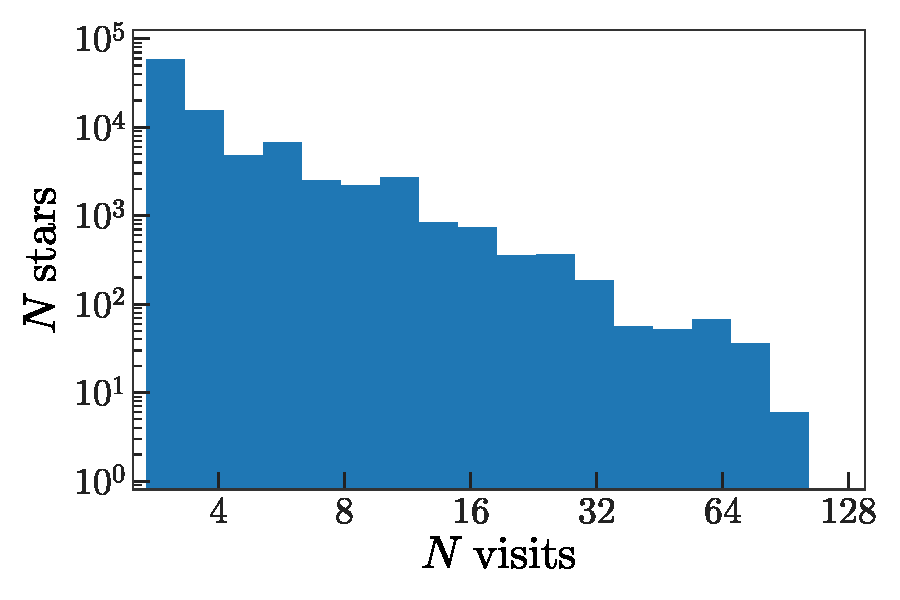
\includegraphics[width=0.7\textwidth]{nvisits.pdf}
\end{center}
\caption{%
Number of \apogee\ stars in logarithmic bins of number of visits that pass the
quality cuts described in \sectionname~\ref{sec:data}.
In total, this work uses \nvisits\ visits and \nstars\ unique sources.
\label{fig:nvisits}
}
\end{figure}

We use the primary data products from \apogee\ \DR\ (i.e. the \texttt{allStar}
and \texttt{allVisit} files) which contain 258,475 unique source IDs
(\texttt{APOGEE\_ID}) and 1,054,381 unique visits.
We select all stars with $\geq 3$ visits that each pass a set of quality cuts,
described below.
For each visit, we require that the visit velocity uncertainty is $< 100~\kms$
(\texttt{VRELERR}) and the following bits are not set in the \texttt{STARFLAGS}
bitmask: \texttt{PERSIST\_HIGH}, \texttt{PERSIST\_JUMP\_POS},
\texttt{PERSIST\_JUMP\_NEG}, \texttt{VERY\_BRIGHT\_NEIGHBOR}, \texttt{LOW\_SNR}.
For each star, we require that $0 < \log g < 4$ and the following bits are not
set in the \texttt{ASPCAPFLAGS} bitmask: \texttt{STAR\_BAD}.
After these cuts, and the requirement of $\geq 3$ visits for a given star, we
are left with \nvisits\ visits for \nstars\ unique sources.
\figurename~\ref{fig:nvisits} shows the number of stars in several bins of
number of visits that pass the above quality cuts: \todo{XX}\% of the stars in
\DR\ have $< 8$ visits.
\figurename~\ref{fig:loggteff} ...

% Notebook: "Numbers of visits and sample overview"
\begin{figure}[h]
\begin{center}
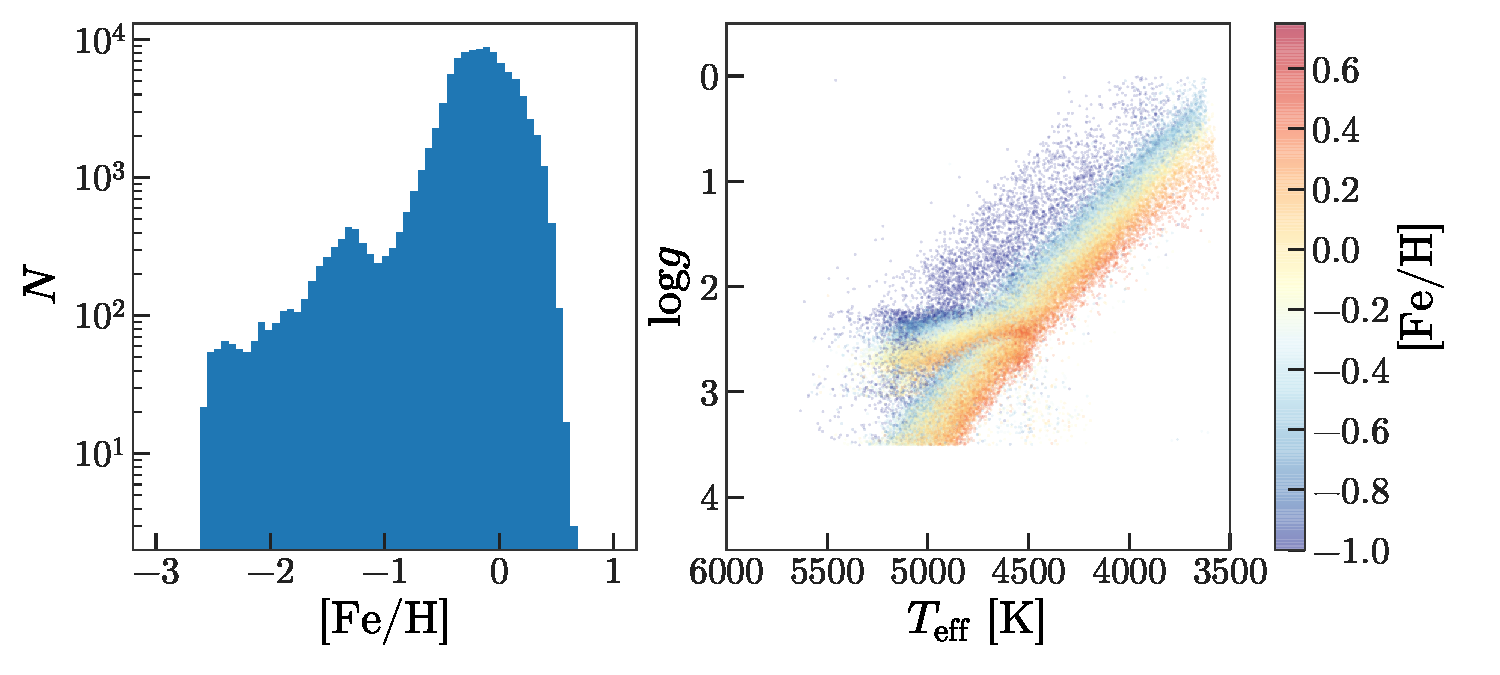
\includegraphics[width=\textwidth]{logg_teff_feh.pdf}
\end{center}
\caption{%
\textit{Left panel}: Number of stars in bins of iron abundance,
$[\textrm{Fe}/\textrm{H}]$, that pass the quality cuts described in
\sectionname~\ref{sec:data}.
\textit{Right panel}: Distribution of stars in our sample in stellar parameters
log-surface-gravity, $\log g$, and effective temperature, $T_{\textrm{eff}}$,
with points colored by the iron abundance.
\label{fig:loggteff}
}
\end{figure}


\section{Methods}

\subsection{Orbit inference and velocity modeling}\label{sec:fitting}

For every source in the sample of \apogee\ stars defined in
\sectionname~\ref{sec:data}, we obtain a posterior sampling in binary-system
parameter space, treating it as a single-lined (SB1) spectroscopic binary system
with a single companion.
This sampling is performed under a relatively uninformative prior pdf, and the
resulting posterior samplings are used to discover and characterize individual
binary-star systems and generate a catalog of companions.
We use \thejoker\ to perform the posterior samplings; we briefly describe the
algorithm below, but a full description is given in previous work
(\citealt{Price-Whelan:2017}).
In this \sectionname, we describe the assumptions and method used to generate
individual-system samplings.

We perform our individual system fits---that is, make our posterior
samplings---under the following assumptions:
\begin{description}
\item[no multiplets] All radial-velocity variations of the primary star are
  induced by a single companion.
  This is motivated by the idea that triple star systems are usually
  hierarchical so that the period of the inner binary is typically much shorter
  than the orbital period of the outer body (\todo{CITATION NEEDED}).
  At present, we ignore the possibility of higher-order multiple systems.
  % \todo{revisit this - do we want to also sample over a long-term trend?}
\item[Kepler] Related to the first point, all velocity variations of the primary
  are gravitational, and we therefore ignore the possibility of coherent intrinsic variation from, e.g., stellar oscillations.
\item[SB1] All spectra are single-lined; that is, we assume that the secondary
  is significantly fainter and is thus undetected in the spectra.
  This assumption is motivated by the fact that we expect \RGB\ stars to be
  substantially more luminous than their typical companion.
  However, there are known main-sequence double-lined binary stars in the
  \apogee\ catalog \citealt{El-Badry:2018}, and an expected but unknown fraction
  of \RGB--\RGB\ binaries.
\item[simple noise model] Measurements are unbiased and noise estimates are
  correct up to an unknown excess variance.
  All noise contributions result in Gaussian uncertainties on the individual
  radial-velocity measurements.
\end{description}

\thejoker\ is a custom-built Monte Carlo sampler designed to produce independent
posterior samples in Keplerian orbital parameters, given radial-velocity
measurements under the assumptions listed above.
Our parametrization of the orbital elements is similar to the notation in
\citet{Murray:2010}:
The radial velocity $v$ at time $t$ is given by
\begin{equation}
  v(t;\bs{\theta}) = v_0 + K\,[\cos\left(\omega + f(t; e, P, M_0, t_0)\right) +
    e\,\cos\omega]
\end{equation}
where $\bs{\theta} = (P,e,M_0,\omega,K,v_0)$---period, eccentricity, mean
anomaly at a reference time $t_0$, argument of pericenter, velocity
semi-amplitude, Barycentric velocity---and the true anomaly, $f$, is a function
of time and the specified parameters (see \sectionname~2 of
\citealt{Price-Whelan:2017} or \eqname~63 in \citealt{Murray:2010}).
In addition to the orbital parameters listed above, \thejoker\ can also generate
samples in an ``excess variance'' parameter, $s^2$, that is added to the
per-visit measurement variances.
This parameter allows us to test whether the visit RV uncertainties are
underestimated
For upper \RGB\ stars the inferred excess variance will be a combination of
extra systematic uncertainty and true astrophysical surface jitter
(\todo{CITATION NEEDED}).

\thejoker\ was designed for the extremely multi-modal pdfs expected when the
number of radial-velocity measurements of a source is small, or the data are
sparse (in phase-coverage) or noisy.
While other Markov Chain Monte Carlo (MCMC) methods have difficulty producing
independent samples with such data, \thejoker\ succeeds by brute force:
After generating an initial (very large) library of prior samples from an
assumed prior pdf (see below), the (typically multi-modal) likelihood is
evaluated at each sample and used to rejection sample.
In practice, given a number of requested samples for each star, the sampling
proceeds iteratively: since it is easier to accept samples when the data is
sparse or noisy, far more prior sample draws (and thus likelihood evaluations)
must occur under very constraining data.

% \subsection{Model selection}
%
% In addition to generating posterior samples for each source, we also compute the
% fully marginalized likelihood (FML) under two other models: (1) a model in which
% the radial velocity of the source is constant, and (2) a model in which the
% radial-velocity variations are purely linear.
% We later use these FML values to define cuts on our full catalog of posterior
% samples to produce a catalog of companions.
%
% \todo{equations?}
%
% Examples of outputs and etc.

\subsection{Individual-system posterior samplings}
\label{sec:samplings}

Here we describe the procedure we use to generate per-target posterior samplings
for the \apogee\ targets.
We execute the full procedure twice for different goals (as described in
\sectionname~\ref{sec:results}), and only here outline the key steps in the
pipeline.

For all \nstars\ \apogee\ stars with $\geq 3$ good visits (see
\sectionname~\ref{sec:data}), we use \thejoker\ to generate posterior samplings
for each star under the assumptions listed above (see
\sectionname~\ref{sec:fitting}).
We start by generating a library of \nprior\ prior samples generated under a
prior similar to that defined in \citet{Price-Whelan:2017}:
\begin{itemize}
    \item uniform or isotropic in angle parameters,
    \item uniform in log-period over the domain $[1,32768]~\textrm{day}$,
    \item a beta distribution over eccentricity with fixed parameters (\citealt{Kipping:2013}).
\end{itemize}
For the prior over the excess variance parameter, $s^2$, we initially use
a Gaussian over the transformed parameter $y = \ln s^2$ with the mean and
standard deviation $(\mu_y, \sigma_y)$ indicated where the runs are described
(see \sectionname~\ref{sec:results}).
The reference time for each star is set to the minimum visit epoch; $M_0$ then
becomes the mean anomaly at the first visit observation.
\tablename~\ref{tbl:params} contains descriptions of all parameters and priors
used.

\begin{table}[h!]
    \centering
    \begin{tabular}{ r c l }
    \hline
    name & prior & description \\
    \hline
    $P$ & $\ln P \sim \mathcal{U}(1, 32768)~\textrm{day}$ & period \\
    $e$ & $e \sim \textrm{Beta}(0.867, 3.03)$ & eccentricity \\
    $t_0$ & fixed & reference time \\
    $M_0$ & $M_0 \sim \mathcal{U}(0, 2\pi)~\textrm{rad}$ & mean anomaly at reference time \\
    $\omega$ & $\omega \sim \mathcal{U}(0, 2\pi)~\textrm{rad}$ & argument of pericenter \\
    $s^2$ & $\ln s^2 \sim \mathcal{N}(\mu_y, \sigma_y^2)$ & extra variance added to each visit variance \\
    $K$ & TODO & velocity semi-amplitude \\
    $v_0$ & TODO & system barycentric velocity \\
    \hline
    \end{tabular}
    \caption{Summary and description of parameters. $\textrm{Beta}(a, b)$ is the beta distribution with \todo{a, b}, $\mathcal{U}(a, b)$ the uniform distribution over the domain $(a, b)$, and $\mathcal{N}(\mu, \sigma^2)$ is the normal distribution with mean $\mu$ and variance $\sigma^2$.}
    \label{tbl:params}
\end{table}

We request \nposterior\ posterior samples for each source.
Depending on the data quality and phase coverage of the visits, \thejoker\ will
require different numbers of prior samples in order to rejection sample down to
the requested number of posterior samples: For few-epoch or noisy RV data, many
prior samples will pass the rejection step, whereas for very precise or
many-epoch RV data, \thejoker\ may need to go process the full library of prior
samples.
We therefore generate the posterior samples using an iterative procedure that
adaptively predicts how many prior samples to test for each star.
For sources with very constraining data, \thejoker\ may return fewer than the
requested number of samples (as few as one sample).
When this occurs, we continue sampling either using standard MCMC, or by
increasing the size of the prior cache and continuing rejection sampling with
\thejoker.


\subsubsection{``Needs MCMC'': Following up \thejoker\ with MCMC}

If just one posterior sample is returned after exhausting the full library of
prior samples, or if multiple (but fewer than \nposterior) are returned that all
lie within a single mode of the posterior pdf, the posterior pdf over orbital
parameters is treated as effectively unimodal: these stars are flagged ``needs
MCMC.''
In this case, we use the location of the returned sample (if only one is
returned), or a randomly chosen sample from those returned (if multiple samples
are returned within one mode) to generate a small Gaussian ball of initial
conditions and use standard MCMC to continue sampling until we obtain
\nposterior\ samples.

We use an ensemble MCMC sampling algorithm (\citealt{Goodman:2010}) implemented
in \python\ (\package{emcee}; \citealt{Foreman-Mackey:2013}) to perform the
samplings.
We transform the standard Keplerian orbital parameters to a safer
parametrization, $(\ln P, \sqrt{K}\,\cos M_0, \sqrt{K}\,\sin M_0, \sqrt{e}\,\cos
\omega, \sqrt{e}\,\cos \omega, \ln s^2, v_0)$, to sample in.
This reparametrization is safer and more efficient for sampling with
\package{emcee}, which expects parameters to be components of a vector so that
linear operations can be applied (see, e.g., \citealt{Hogg:2017}); the angle
variables $(\omega, M_0)$ don't meet this requirement in the standard
parametrization.
We use the same prior pdfs as in \thejoker\ when running MCMC (see
\tablename~\ref{tbl:params}).

For each star that is flagged ``needs MCMC,'' we run \package{emcee} with 1024
walkers for 16384 steps, take the final walker positions, and downsample at
random until we have \nposterior\ samples.
We compute the Gelman--Rubin convergence statistic, $\hat{R}_j$,
(\citealt{Gelman:1992}) for each parameter $j$ and include these values in the
catalogs below when standard MCMC is run.
We also provide a binary flag, ``converged,'' for each sampling continued with
MCMC that is set to true if:
\begin{equation}
\underset{j}{\textrm{mean}}\left(\hat{R}_j\right) < 1.1 \quad .
\end{equation}


\subsubsection{``Needs more prior samples'': Continuing \thejoker\ sampling}

If more than one posterior sample is returned after exhausting the full library
of prior samples, and the samples lie in multiple modes of the posterior pdf,
the only way to proceed is to generate more prior samples and continue running
\thejoker: these stars are flagged ``needs more prior samples.''
In this case, we generate another equal-sized library of prior samples (a total
of $2\times\nprior$ samples) and re-do the rejection sampling.
We note that because of the way the rejection sampling step is done, this is not
equivalent to concatenating the results from a second, independent run of
\thejoker: the log-likelihood values for all of the prior samples must be used.
If at the end of this second run the target still has fewer than \nposterior\
samples, the sampling is flagged as ``incomplete.''

\subsection{Implementation notes}

\todo{Nontrivial computation - details about running on cluster, TheJoker vs. emcee}

\section{Experiment: infer the excess variance distribution}
\label{sec:inferjitter}

\todo{Fix this bit from copy-pasting}

A full run of \thejoker\ on all \nstars\ \apogee\ stars used in this work took
approximately 300 hours on a compute cluster with 448 cores, with the time
dominated by sources with many ($\gtrsim 10$) visits.

For this initial run, we do not follow up on stars that return $<$\nposterior\
samples.

of the initial distribution set to $(\mu_{y,0}, \sigma_{y,0})
= (10.6, 3)$ in units of $\textrm{m}~\textrm{s}^{-1}$.

As an initial use of the per-source posterior samplings, we use a hierarchical
Bayesian model to infer the parameters of the (assumed Gaussian) prior over the
log-excess-variance parameter, $(\mu_y, \sigma_y)$ (see
\tablename~\ref{tbl:params}).
This inference serves as a test-case for future work, where we intend to use the
independent posterior samplings to construct a hierarchical inference over
companion population properties.
This is also a test of the visit velocity uncertainties reported in the \apogee\
data products: If the catalog uncertainties are significantly underestimated, we
expect the inferred log-excess-variance distribution parameters to tend towards
larger values.

In detail, we maximize the marginal likelihood of the population-level
parameters $(\mu_y, \sigma_y)$.
We compute this marginal likelihood using the per-object posterior samples
re-weighted by the ratio of the value of the hyperprior evaluated at a given,
new set of parameters $(\mu_y, \sigma_y)$ over the value of the default prior at
the previously assumed values, $(\mu_{y,0}, \sigma_{y,0})$ (see above).
This trick has been used in other hierarchical inferences as a way to
marginalize over the per-object parameters to infer population-level parameters
(\citealt{Hogg:2010,Foreman-Mackey:2014}); we describe how to compute the
marginal likelihood in detail in \sectionname~\ref{sec:hierarch}.

We use 1,825 stars with $>10$ visits and $\log g < 2$ (to avoid upper RGB stars
that have large intrinsic jitter) and maximize the above likelihood to determine
better hyperparameters for the log-excess-variance parameter distribution.
\figurename~\ref{fig:infer-jitter} shows the distribution corresponding to the
maximum-likelihood hyperparameters, $\alpha^* = (\mu_y^*, \sigma_y^*) = (9.50,
1.64)$.
\todo{Reactions to the inferred parameters?}

% Notebook: "Infer jitter"
\begin{figure}[h]
\begin{center}
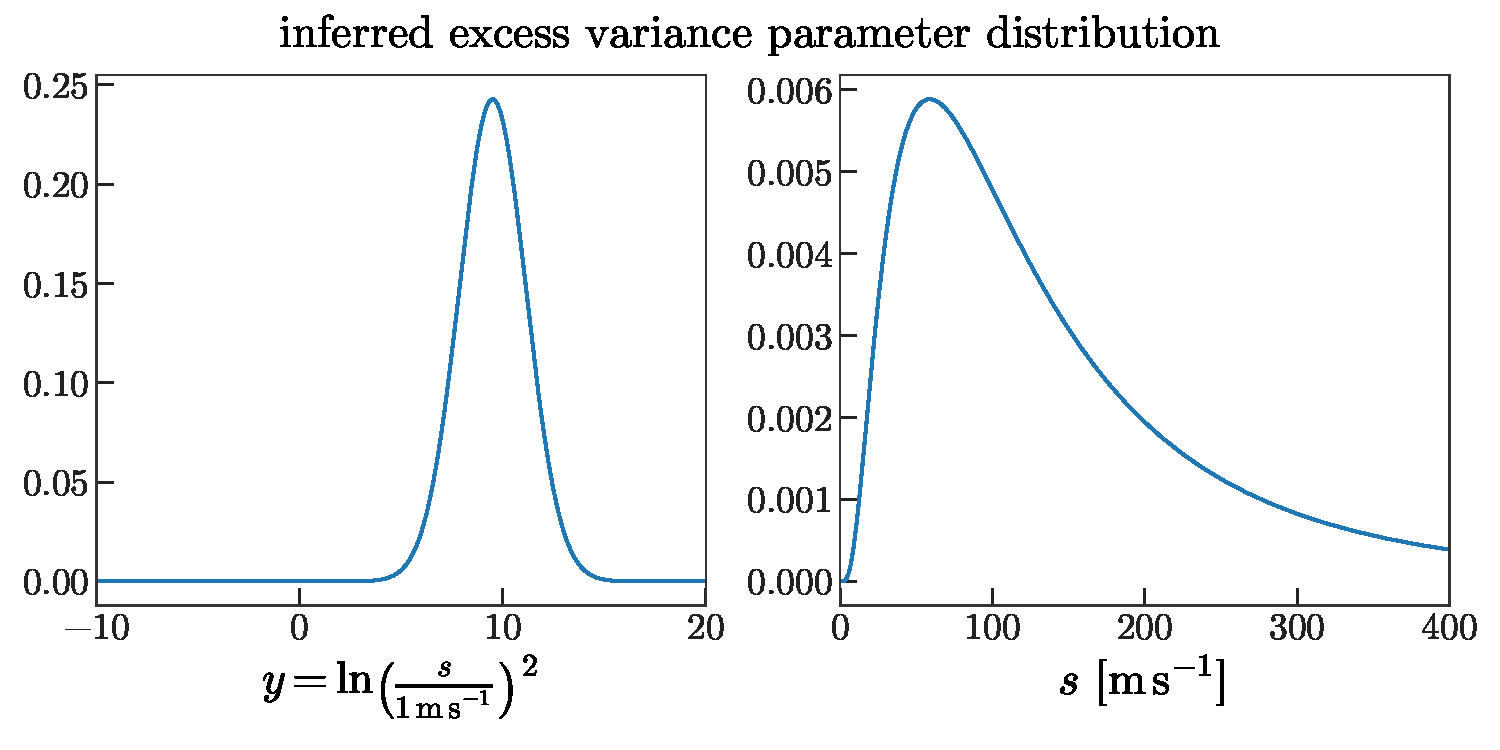
\includegraphics[width=\textwidth]{infer-jitter}
\end{center}
\caption{%
\todo{move notebook to figures path, re-do with "run2" or "run1" samples...}
Inferred prior over log-jitter parameter ($y = \ln s^2$) using posterior samples
for 1,825 lower-RGB stars with $>10$ visits.
Left panel shows the ... Right panel shows the ...
\label{fig:infer-jitter}
}
\end{figure}

\section{Results: companion catalogs}
\label{sec:results}

Using the maximum-likelihood hyperparameters derived from the initial posterior
samplings (see \sectionname~\ref{sec:initsampling}), we update and fix the
excess variance prior distribution parameters---$(\mu_{y}, \sigma_{y}) = (9.5,
1.6)$ in units of $\textrm{m}~\textrm{s}^{-1}$---and re-run \thejoker\ on the
parent sample of \apogee\ \DR\ stars.
\todo{Discuss how this relates to empirical Bayes?}

From this run, 91,096 stars completed and successfully returned \nposterior\
samples using \thejoker\ alone.
The remaining 5,135 stars did not return \nposterior\ samples: 4,744 were
flagged as \emph{needs more prior samples}, 391 as \emph{needs MCMC}.

\todo{Stuff about full catalog of posterior samples, available online}

\subsection{Stars with confident companions}
\label{sec:catalog-confident}

\todo{Thresholding on what now?}

\todo{Examples of stars with no companions at various num. epochs}

\todo{Examples of stars that meet K cut at various num. epochs}

\subsection{Confident companions with highly constrained orbits}
\label{sec:catalog-multimodal}

\todo{Many examples of stars that meet K cut but solutions limited to a few
qualitatively different solutions}

\subsection{Confident companions with effectively uniquely determined orbits}
\label{sec:catalog-unimodal}

\todo{Many examples of stars that are probably unimodal}

\todo{Period - eccentricity plot? Tidal circularization (See "Debug MCMC
continue")}

\todo{Stars with Martig or Ness masses - m2min}

\section{Discussion}

\todo{Return to our various assumptions and make sure that we discuss them
\emph{by name} here.}

\subsection{Comparison to other APOGEE companion catalogs}
\label{sec:compare-troup}

There are at least two other recent catalogs of stellar systems and companions
based on \apogee\ data.

One of these studies focused on decomposing spectra of MS stars into mixtures of
stellar spectra (\citealt{El-Badry:2018}).
Conceptually, this method works because (a) for two unequal-mass stars,
unexpected absorption lines will appear superimposed on the brighter star's
spectrum, and (b) for close to equal-mass stars, the line depths and ratios will
not be well-matched by a single stellar model.
Using this technique, they identified thousands of candidate MS binaries and
trinaries, but did not consider giant stars ($\log g > 4$).
This sample is therefore complimentary to and non-overlapping with the catalog
presented in this work.

The other recent catalog searched for stellar and substellar companions to all
stars in \apogee\ \acronym{DR12} (including the RGB) that passed a series of
quality cuts, and had $\geq 8$ visits (\citealt{Troup:2016}).
For each star in the sample, orbits were fit to the visit RVs using a multi-step
orbit-fitting procedure: it starts by identifying significant periods and a few
harmonics of those periods, then fits a Keplerian orbit at each of these
harmonics using least-squares fitting (\citealt{De-Lee:2013}) with a modified
$\chi^2$ statistic that penalizes fits in which the phase coverage of the data
is poor.
This procedure is not guaranteed to provide a unique orbit solution.

Of the 382 companions released as a part of this previous search, only 188 of
the host stars passed the stellar parameter and quality cuts used to define the
parent sample in this work (see \sectionname~\ref{sec:data}).
We have looked at all of the overlapping stars to compare the previously derived
companion orbital properties to the posterior samplings derived with \thejoker.
We find that the comparisons fall in three categories:
(1) the parameters reported in \citet{Troup:2016} agree with the posterior
samplings, and the period distribution appears unimodal,
(2) the parameters reported in \citet{Troup:2016} identify one possible mode of
a likely multi-modal posterior pdf over orbital parameters, and
(3) the data changed significantly between \apogee\ \acronym{DR12} and \DR, so
no meaningful comparisons can be made; Roughly 1/3 of the comparison sample
falls into each class.
\figurename~\ref{fig:troup-unimodal} shows a few representative cases in which
the \citet{Troup:2016} orbital parameters (orbit shown as orange line in left
panels, parameters shown as orange + in right panels) is consistent with the
orbit samples from \thejoker.
\figurename~\ref{fig:troup-multimodal} shows a few representative cases in which
we find that the posterior pdf over orbital parameters is multimodal, and the
\citet{Troup:2016} orbit identifies one of these modes.
For completeness, \figurename~\ref{fig:troup-datachanged} shows two instances in
which the orbital parameters from \citet{Troup:2016} no longer make sense,
likely because the data changed between data releases.

\begin{figure}[h]
\begin{center}
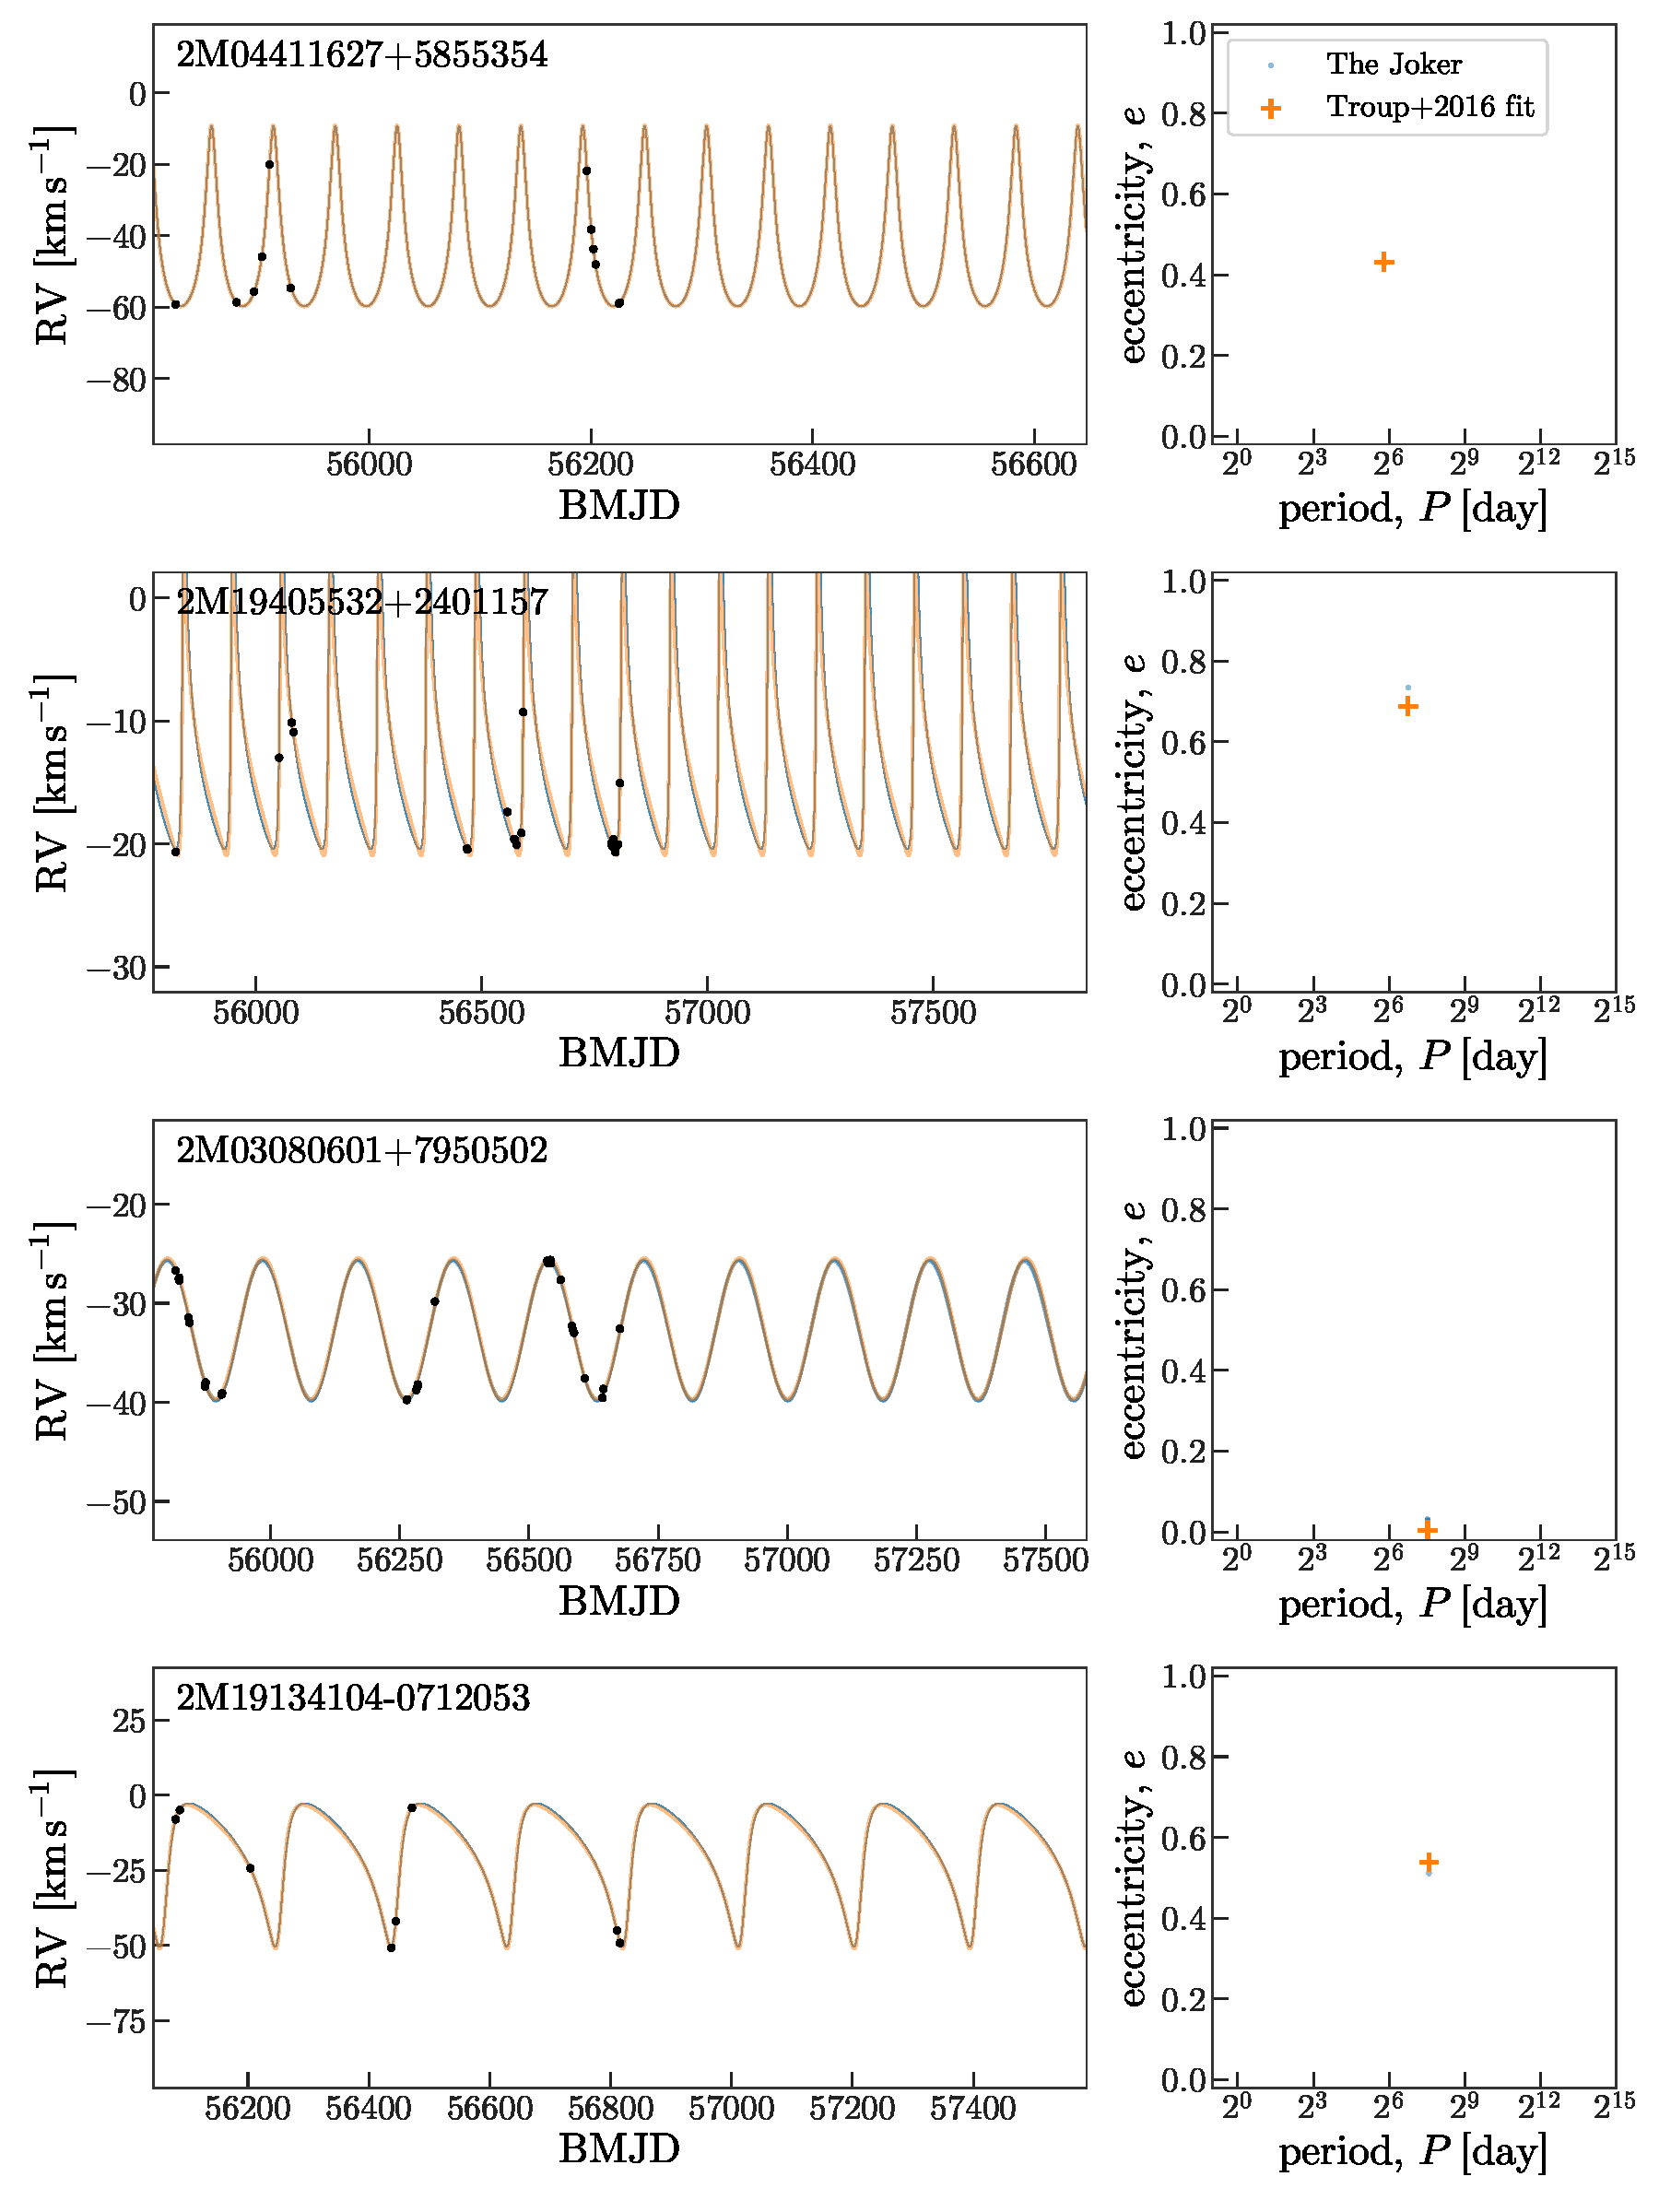
\includegraphics[width=\textwidth]{unimodal.pdf}
\end{center}
\caption{%
TODO:
\label{fig:troup-unimodal}
}
\end{figure}

\begin{figure}[h]
\begin{center}
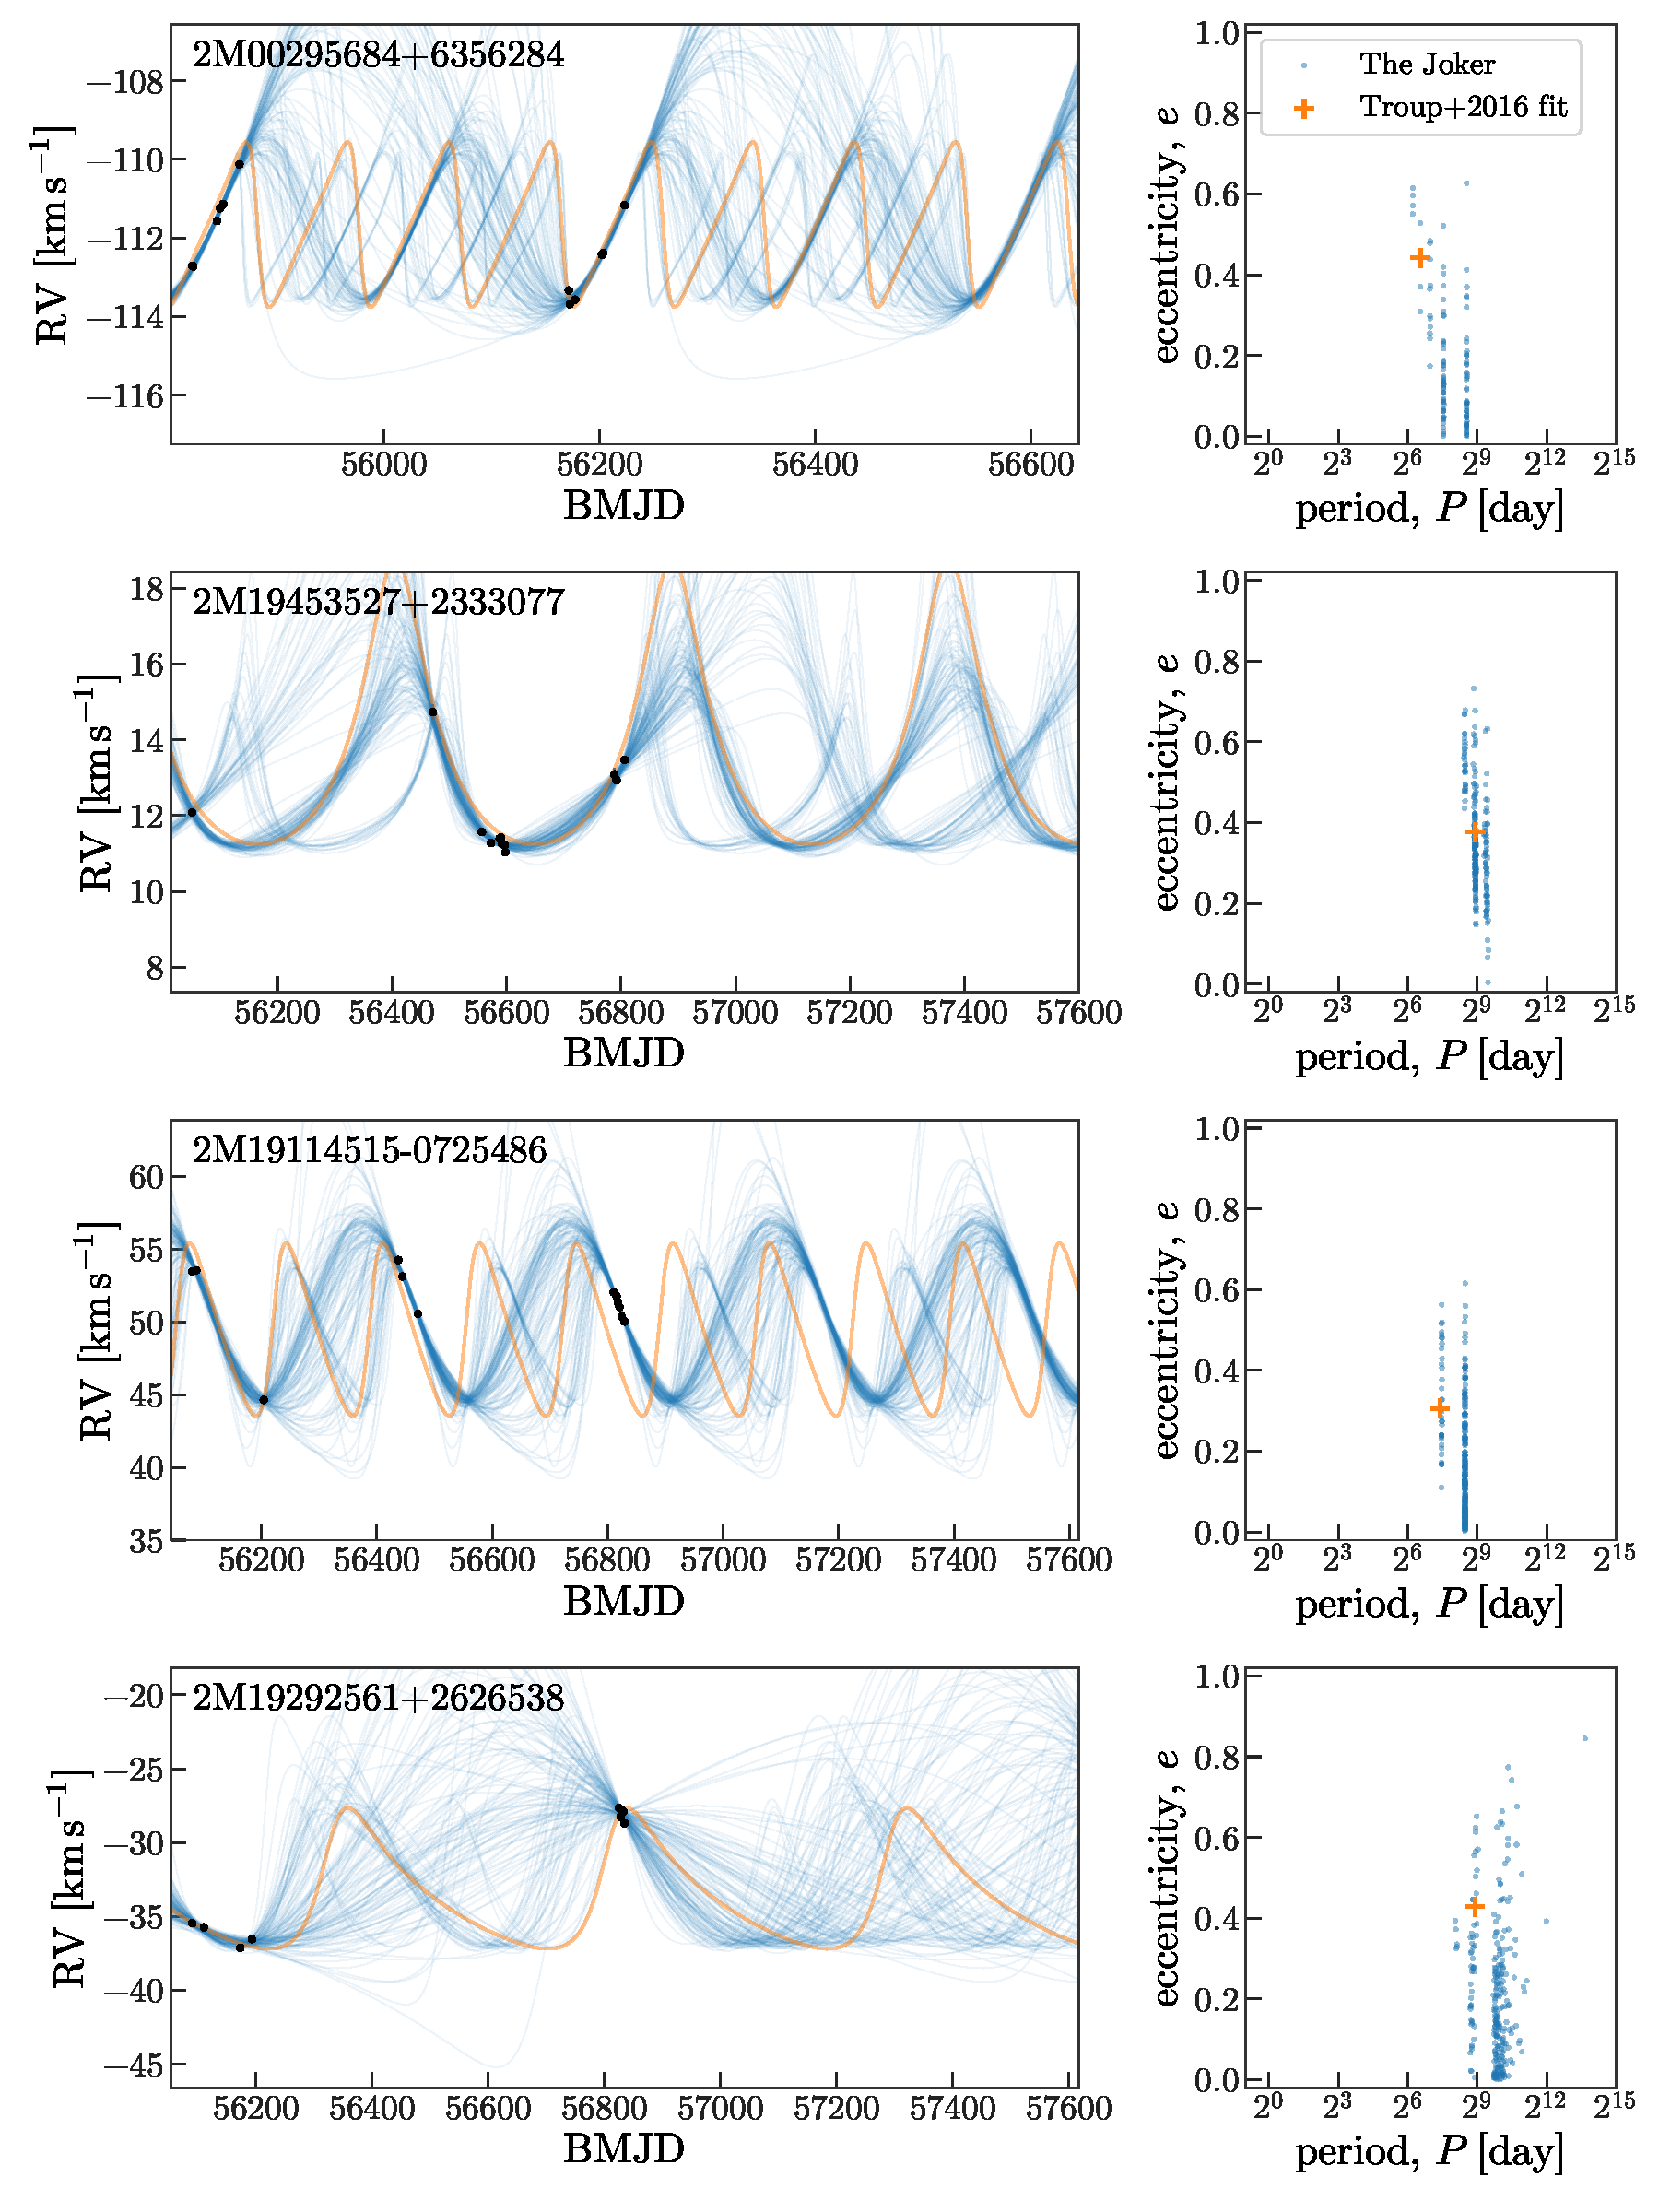
\includegraphics[width=\textwidth]{multimodal.pdf}
\end{center}
\caption{%
TODO:
\label{fig:troup-multimodal}
}
\end{figure}

\begin{figure}[h]
\begin{center}
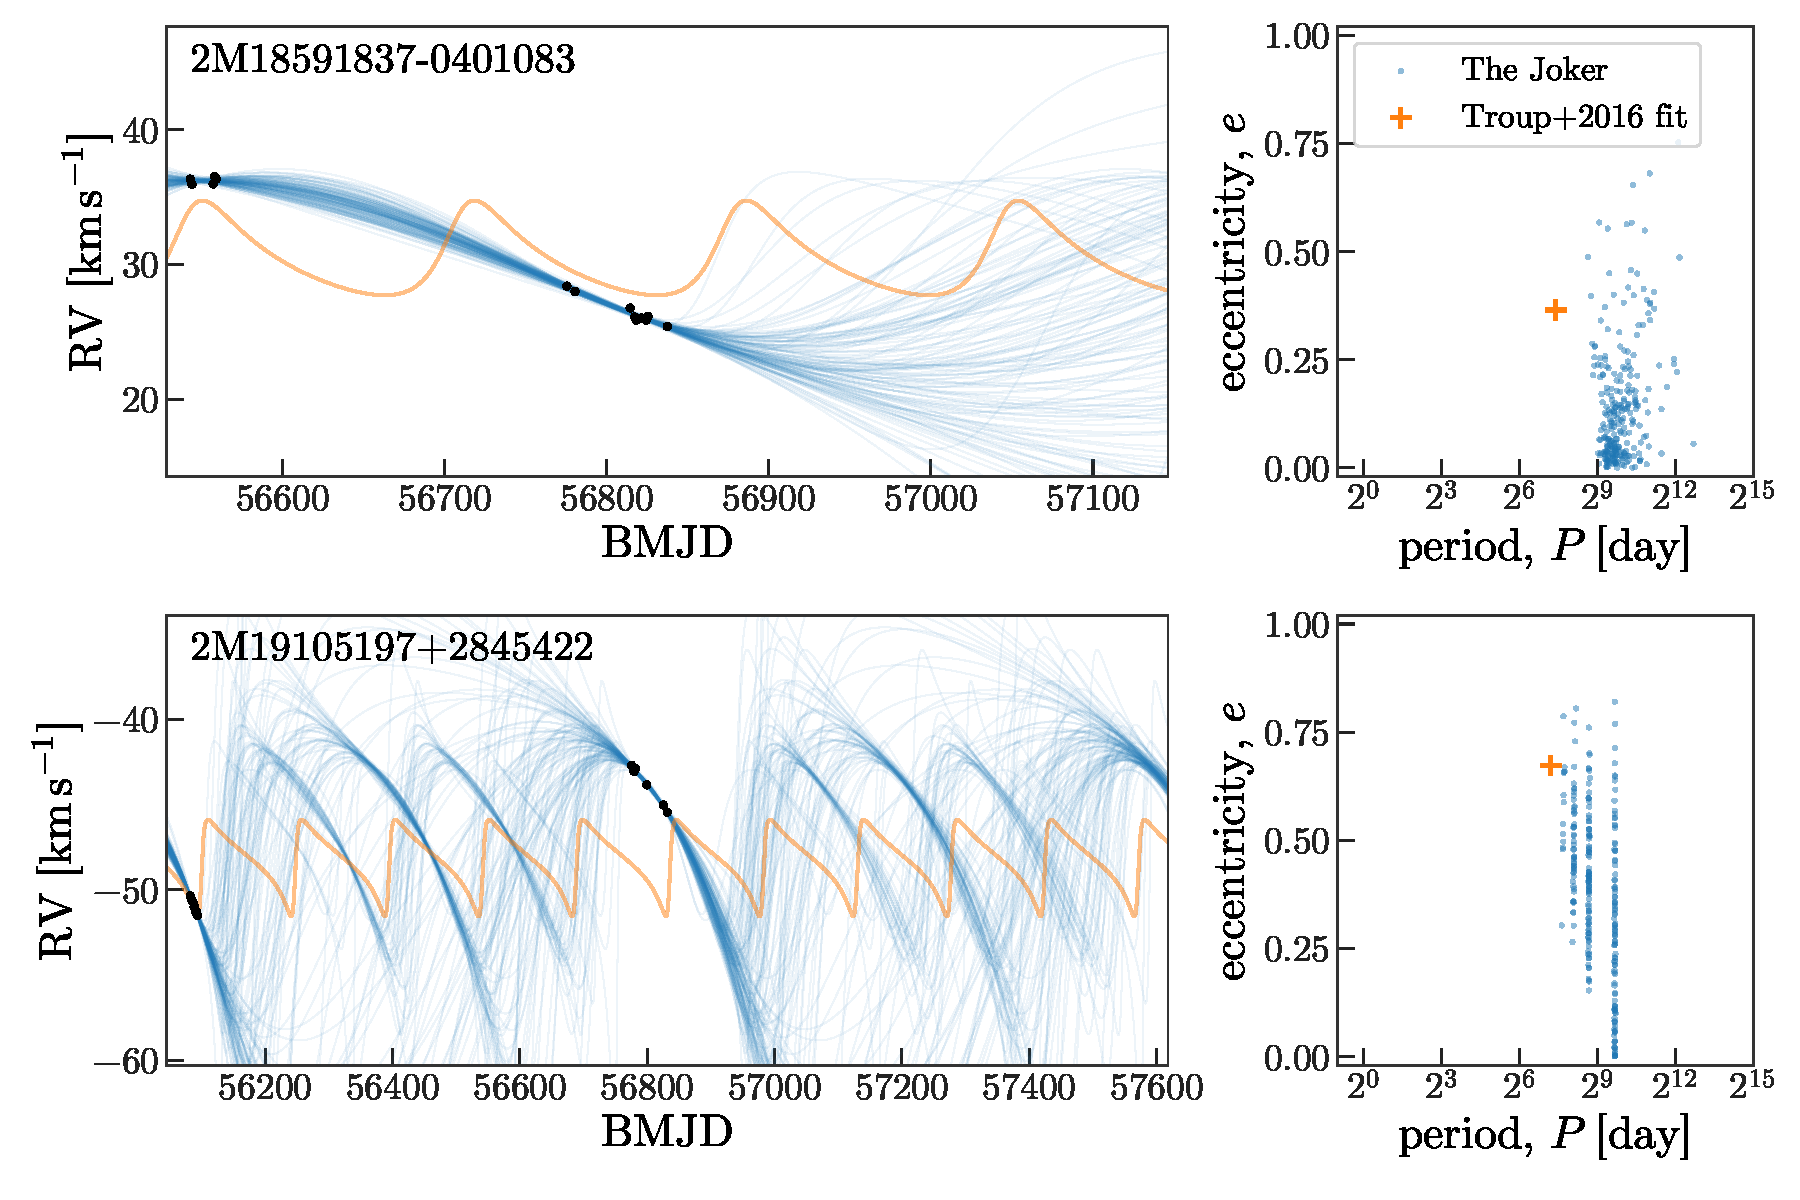
\includegraphics[width=\textwidth]{data-changed.pdf}
\end{center}
\caption{%
TODO:
\label{fig:troup-datachanged}
}
\end{figure}

\subsection{Population inference}

Comment on things we could do with these samples hierarchical inference...

We are SB1 only, but should do SB2 as well - no reason to restrict.

\section{Conclusions}

Tables available online, full code open source.\footnote{The code used in this
project is available from \url{https://github.com/adrn/TwoFace} under the MIT
open-source software license.}

\acknowledgements

It is a pleasure to thank Keith Hawkins (Columbia), XXXXXXX.

The authors are pleased to acknowledge that the work reported on in this
paper was substantially performed at the TIGRESS high performance computer
center at Princeton University which is jointly supported by the Princeton
Institute for Computational Science and Engineering and the Princeton
University Office of Information Technology's Research Computing department.

\software{
    \package{Astropy} (\citealt{Astropy-Collaboration:2013}),
    \package{emcee} (\citealt{Foreman-Mackey:2013}),
    \package{IPython} (\citealt{Perez:2007}),
    \package{matplotlib} (\citealt{Hunter:2007}),
    \package{numpy} (\citealt{Van-der-Walt:2011}),
    \package{scipy} (\url{https://www.scipy.org/}),
    \package{sqlalchemy} (\url{https://www.sqlalchemy.org/}).
}

\facility{\sdssiv, \apogee}

\bibliographystyle{aasjournal}
\bibliography{refs}

\appendix
\section{Hierarchical inference of the excess variance parameter}
\label{sec:hierarch}

For each $n$ of $N$ RGB stars in APOGEE, we obtain $K$ posterior samples over
primary orbital parameters $\bs{\theta} = (P, e, \omega, M_0, K, v_0)$ and the
excess-variance parameter, $y = \ln s^2$, using \thejoker; For brevity in
expressions below, we will use the vector
\begin{equation}
    \bs{w} = (\bs{\theta}, y)
\end{equation}
to represent the full set of parameters.
To obtain this sampling, we use an interim (Gaussian) prior on the
excess-variance parameter parametrized by a mean and standard deviation, i.e.
$\alpha_0 = (\mu_{y,0}, \sigma_{y,0})$ as described above.
For a given source, the posterior samples in the above parameters are drawn from
the distribution
\begin{equation}
    \bs{w}_k \sim p(\bs{w}_k \given D, \bs{\alpha}_0)
\end{equation}
where $D$ represents the data for a given object.

We want to compute the likelihood of all data from all $N$ stars, $\{D_n\}$,
given a new set of hyperparameters $\bs{\alpha}$
\begin{equation}
    p(\{D_n\} \given \bs{\alpha}) = \prod_n^N p(D_n \given \bs{\alpha})
\end{equation}
where in the above, we have assumed that this likelihood is separable ( the data
for each source are independent).
The per-source marginal likelihood in the above expression is given by
\begin{align}
    p(D_n \given \bs{\alpha}) &= \int \dd \bs{w}_n \, p(D_n \given \bs{w}_n) \,
      p(\bs{w}_n \given \bs{\alpha})\\
    &= \int \dd \bs{w}_n \, p(D_n \given \bs{w}_n) \, p(\bs{w}_n \given \bs{\alpha}) \,
      \frac{p(\bs{w}_n \given D_n, \bs{\alpha}_0)}{p(\bs{w}_n \given D_n, \bs{\alpha}_0)}\\
    &= p(D_n \given \bs{\alpha}_0) \, \int \dd \bs{w}_n \,
      \frac{p(\bs{w}_n \given \bs{\alpha})}{p(\bs{w}_n \given \bs{\alpha}_0)} \,
      p(\bs{w}_n \given D_n, \bs{\alpha}_0) \label{eq:marglike} \quad .
\end{align}
Using the Monte Carlo integration approximation, \eqname~\ref{eq:marglike} can
be simplified to a sum over prior value ratios of the $K$ posterior samples in
the log-excess-variance parameter for each $n$ star
\begin{equation}
    \approx \frac{\mathcal{Z}_n}{K} \,
      \sum_k^{K} \frac{p(y_{nk} \given \bs{\alpha})}{p(y_{nk} \given \bs{\alpha}_0)}
\end{equation}
where we have canceled the other priors (over $\bs{\theta}$), and all
normalization constants appear in the constant scale factor $\mathcal{Z}_n$.

The above expresion gives the marginal likelihood of the velocity data for a single source given new hyperparameters $\bs{\alpha}$.
The full marginal likelihood is then the product of these individual likelihoods
\begin{align}
    p(\{D_n\} \given \alpha) &\propto \prod_n^N \frac{1}{K} \,
      \sum_k^{K} \frac{p(y_{nk} \given \alpha)}{p(y_{nk} \given \alpha_0)}
      \quad .
\end{align}
In practice, we evaluate the log-marginal-likelihood
\begin{align}
    \ln p(\{D_n\} \given \alpha) &\propto \sum_n^N \left[
      \ln\left( \sum_k^{K} \frac{p(y_{nk} \given \alpha)}{p(y_{nk} \given \alpha_0)} \right)
      - \ln K\right]\label{eq:lnlike}\\
    &\propto \sum_n^N \left[
      \underset{k}{\textrm{logsumexp}}\left[ \ln{p(y_{nk} \given \alpha)} - \ln{p(y_{nk} \given \alpha_0)} \right]
      - \ln K\right]
\end{align}
where $\textrm{logsumexp}$ (the log-sum-exp trick) provides a more stable
estimate of the sum in \eqname~\ref{eq:lnlike}.

\end{document}
